\documentclass{article}

\usepackage{fancyhdr}
\usepackage{extramarks}
\usepackage{amsmath,mathrsfs,amssymb}
\usepackage{amsthm}
\usepackage{amsfonts}
\usepackage{tikz}
\usepackage[plain]{algorithm}
\usepackage{algpseudocode}
\usepackage[]{mcode}
\usepackage{graphicx}
\usepackage{pgfplots}
\usepackage{xfrac,siunitx}
\usepackage{gensymb}
\usepackage{caption}
\usepackage{epstopdf}

\usetikzlibrary{automata,positioning}
\usetikzlibrary{calc}
\usetikzlibrary{shapes,arrows}

%
% Basic Document Settings
%

\topmargin=-0.45in
\evensidemargin=0in
\oddsidemargin=0in
\textwidth=6.5in
\textheight=9.0in
\headsep=0.25in

\linespread{1.1}

\pagestyle{fancy}
\lhead{\hmwkAuthorName}
\chead{\hmwkClass\ (\hmwkClassInstructor\ \hmwkClassTime): \hmwkTitle}
\rhead{\firstxmark}
\lfoot{\lastxmark}
\cfoot{\thepage}

\renewcommand\headrulewidth{0.4pt}
\renewcommand\footrulewidth{0.4pt}

\setlength\parindent{0pt}

%
% Create Problem Sections
%

\newcommand{\enterProblemHeader}[1]{
    \nobreak\extramarks{}{Problem \arabic{#1} continued on next page\ldots}\nobreak{}
    \nobreak\extramarks{Problem \arabic{#1} (continued)}{Problem \arabic{#1} continued on next page\ldots}\nobreak{}
}

\newcommand{\exitProblemHeader}[1]{
    \nobreak\extramarks{Problem \arabic{#1} (continued)}{Problem \arabic{#1} continued on next page\ldots}\nobreak{}
    \stepcounter{#1}
    \nobreak\extramarks{Problem \arabic{#1}}{}\nobreak{}
}

\setcounter{secnumdepth}{0}
\newcounter{partCounter}
\newcounter{homeworkProblemCounter}
\setcounter{homeworkProblemCounter}{1}
\nobreak\extramarks{Problem \arabic{homeworkProblemCounter}}{}\nobreak{}

%
% Homework Problem Environment
%
% This environment takes an optional argument. When given, it will adjust the
% problem counter. This is useful for when the problems given for your
% assignment aren't sequential. See the last 3 problems of this template for an
% example.
%
\newenvironment{homeworkProblem}[1][-1]{
    \ifnum#1>0
        \setcounter{homeworkProblemCounter}{#1}
    \fi
    \section{Problem \arabic{homeworkProblemCounter}}
    \setcounter{partCounter}{1}
    \enterProblemHeader{homeworkProblemCounter}
}{
    \exitProblemHeader{homeworkProblemCounter}
}

%
% Homework Details
%   - Title
%   - Due date
%   - Class
%   - Section/Time
%   - Instructor
%   - Author
%

\newcommand{\hmwkTitle}{Tutorial\ 2}
\newcommand{\hmwkDueDate}{August 09, 2016}
\newcommand{\hmwkClass}{Control Engineering}
\newcommand{\hmwkClassTime}{}
\newcommand{\hmwkClassInstructor}{Professor Friso De Boer}
\newcommand{\hmwkAuthorName}{S.Reynolds (262538)}

%
% Title Page
%

\title{
    \vspace{2in}
    \textmd{\textbf{\hmwkClass:\ \hmwkTitle}}\\
    \normalsize\vspace{0.1in}\small{Due\ on\ \hmwkDueDate\ at 3:00pm}\\
    \vspace{0.1in}\large{\textit{\hmwkClassInstructor\ \hmwkClassTime}}
    \vspace{3in}
}

\author{\textbf{\hmwkAuthorName}}
\date{}

\renewcommand{\part}[1]{\textbf{\large Part \Alph{partCounter}}\stepcounter{partCounter}\\}

%
% Various Helper Commands
%

% Useful for algorithms
\newcommand{\alg}[1]{\textsc{\bfseries \footnotesize #1}}

% For derivatives
\newcommand{\deriv}[1]{\frac{\mathrm{d}}{\mathrm{d}x} (#1)}

% For partial derivatives
\newcommand{\pderiv}[2]{\frac{\partial}{\partial #1} (#2)}

% Integral dx
\newcommand{\dx}{\mathrm{d}x}

% Alias for the Solution section header
\newcommand{\solution}{\textbf{\large Solution}}

% Probability commands: Expectation, Variance, Covariance, Bias
\newcommand{\E}{\mathrm{E}}
\newcommand{\Var}{\mathrm{Var}}
\newcommand{\Cov}{\mathrm{Cov}}
\newcommand{\Bias}{\mathrm{Bias}}

\DeclareMathOperator{\sinc}{sinc}

\graphicspath{{./fig/}}

\begin{document}

\maketitle

\pagebreak

%%%%%%%%%%%%%%%%%%%%%%%%%%%%%%%%%%%%%%%%%%%%%%%%%%%%%%%%%%%%%%%%%%%%%%%%%%%%%%%%%%%%%%%%%%%%%%%%%%%%%%%%%%%%%%%%%%%%%%
% Question 2.1
%%%%%%%%%%%%%%%%%%%%%%%%%%%%%%%%%%%%%%%%%%%%%%%%%%%%%%%%%%%%%%%%%%%%%%%%%%%%%%%%%%%%%%%%%%%%%%%%%%%%%%%%%%%%%%%%%%%%%% 


    \textbf{Question 2.1}\\
    
     Consider the picture below. The force which controls the direction about the centre of gravity of the rocket is the force which acts orthogonal to the centre line down the body of the rocket. We note that the force from the engine, $\vec{F}$, makes an angle with the centre line of $\alpha$.
    
    %%%%%%%%%%%%%%%%%%%%%%%%%%%%%%%%%%%%%%%%%%%%%%%%%%%%%%%%%%%%%%%%
    
    % Code which helps put in angle arcs
    
    \newcommand{\tikzAngleOfLine}{\tikz@AngleOfLine}
    \def\tikz@AngleOfLine(#1)(#2)#3{%
    	\pgfmathanglebetweenpoints{%
    		\pgfpointanchor{#1}{center}}{%
    		\pgfpointanchor{#2}{center}}
    	\pgfmathsetmacro{#3}{\pgfmathresult}%
    }
    %%%%%%%%%%%%%%%%%%%%%%%%%%%%%%%%%%%%%%%%%%%%%%%%%%%%%%%%%%%%%%%%
    
    \begin{figure}[h]
    	\centering
    	\begin{tikzpicture}[scale = 0.5]
    	% Draw the axes of the figure
    	\draw [dashed,<-,cm={cos(45) ,-sin(45) ,sin(45) ,cos(45) ,(0 cm,0 cm)}](-5,0) coordinate (F) node[above] {$y$} -- (0,0) coordinate (A) node[] {} -- (5,0) coordinate (B) node[] {}; %x-axis
    	\draw [dashed,->,cm={cos(45) ,-sin(45) ,sin(45) ,cos(45) ,(0 cm,0 cm)}](0,-5) -- (0,5) node[above] {$x$}; %y-axis
    	
    	% Draw the body of the rocket
    	\draw[cm={cos(45) ,-sin(45) ,sin(45) ,cos(45) ,(0 cm,0 cm)}] (2,0.5) -- (2,-0.5) -- (-4,-0.5) -- (-4,0.5) -- (2,0.5);
    	
    	% Draw the force vector in blue
    	\draw[-latex,blue,cm={cos(45) ,-sin(45) ,sin(45) ,cos(45) ,(0 cm,0 cm)}] (4,-1) coordinate (C) node[below] {$\vec{F}$} -- (2,0) coordinate (D) node[] {};
    	
    	% Draw the reference line through the centre of gravity
    	\draw [dashed] (0,-2) -- (0,4) coordinate (E) node[]{};
    	
    	\tikzAngleOfLine(D)(C){\AngleStart}
    	\tikzAngleOfLine(D)(B){\AngleEnd}
    	\draw[red,<->] (D)+(\AngleStart:2cm) arc (\AngleStart:\AngleEnd:2 cm);
    	\node[] at ($(D)+({(\AngleStart+\AngleEnd)/2}:1.35 cm)$) {$\alpha$};
    	
    	\tikzAngleOfLine(A)(E){\AngleStart}
    	\tikzAngleOfLine(A)(F){\AngleEnd}
    	\draw[red,<->] (A)+(\AngleStart:2.5cm) arc (\AngleStart:\AngleEnd:2.5cm);
    	\node[] at ($(A)+({(\AngleStart+\AngleEnd)/2}:3.2 cm)$) {$\phi (t)$};
    	
    	\fill (0,0) circle[radius=3pt] node[label={[label distance=0.15cm]3:$C$}]{};
    	
    	\end{tikzpicture}
    \end{figure}
    
    
    We also note that the direction of the rocket can be specified using the parameter $\phi$, which is the angle between the vertical reference line and the centre line of the rocket. Decomposing the force into components which run along the line, and are orthogonal to the line yield the following results:
    \begin{align*}
	    \vec{F}_{parallel} &= \vec{F} \cdot \cos (\alpha)\\
	    \vec{F}_{orthogonal} &= \vec{F} \cdot \sin (\alpha)
    \end{align*}
	
	Now, if we consider the moment about the centre of gravity of the rocket, $C$, then we can express this in two different ways:
	\begin{align}
		\vec{M}_C &= \vec{F} \cdot \sin (\alpha) \cdot 0.4 \times l\\
		\vec{M}_C &= J \cdot \ddot{\phi}
	\end{align}

	Rearranging equation (2), and substituting equation (1), we obtain the following differential equation:
	\begin{align}
		\ddot{\phi} = \frac{1}{J} \cdot \vec{F} \cdot \sin (\alpha) \cdot 0.4 \times l
	\end{align}
	
	Equation (3) is a non-linear differential equation, and if we assume that $\alpha$ is small, we note that $\sin (\alpha) \approx \alpha$, and hence we get the equation:
	\begin{align}
		\ddot{\phi} = \frac{1}{J} \cdot \vec{F} \cdot \alpha \cdot 0.4 \times l
	\end{align}
	
	Given that $J = 1 \times 10^{-6} \ \si{\newton\meter\second^2}$, $\vec{F} = 100 \ \si{\newton}$, and the length of the rocket is $25 \ \si{\meter}$, equation (4) becomes:
	\begin{align}
		\ddot{\phi}(t) = \alpha (t)
	\end{align}
	
	
%%%%%%%%%%%%%%%%%%%%%%%%%%%%%%%%%%%%%%%%%%%%%%%%%%%%%%%%%%%%%%%%%%%%%%%%%%%%%%%%%%%%%%%%%%%%%%%%%%%%%%%%%%%%%%%%%%%%%%
% Question 2.2
%%%%%%%%%%%%%%%%%%%%%%%%%%%%%%%%%%%%%%%%%%%%%%%%%%%%%%%%%%%%%%%%%%%%%%%%%%%%%%%%%%%%%%%%%%%%%%%%%%%%%%%%%%%%%%%%%%%%%%

 
    \textbf{Question 2.2}\\
    
    To find the transfer function of the differential equation show in equation (5), we take the Laplace transform:
    \begin{align*}
	    \mathscr{L}\{\ddot{\phi}(t)\} = \mathscr{L}\{\alpha (t)\}
    \end{align*}
	
	Hence, we get the following:
	\begin{align*}
		s^2 \cdot \Phi(s) - s \cdot \phi(0) - \dot{\phi}(0) = A(s)
	\end{align*}
	
	It is safe to assume that prior to the force from the propulsion being applied, the angle of the rocket with the vertical reference line is zero, and that the rate at which this angle is changing is also zero. Essentially, we are assuming that $\phi(0) = \dot{\phi}(0) = 0$, which yields:
	\begin{align*}
		s^2 \cdot \Phi(s) = A(s)
	\end{align*}
	
	Rearranging, we get the transfer function for the system:
	\begin{align}
		\frac{\Phi (s)}{A(s)} = \frac{1}{s^2}
	\end{align}
	
%%%%%%%%%%%%%%%%%%%%%%%%%%%%%%%%%%%%%%%%%%%%%%%%%%%%%%%%%%%%%%%%%%%%%%%%%%%%%%%%%%%%%%%%%%%%%%%%%%%%%%%%%%%%%%%%%%%%%%
% Question 2.3
%%%%%%%%%%%%%%%%%%%%%%%%%%%%%%%%%%%%%%%%%%%%%%%%%%%%%%%%%%%%%%%%%%%%%%%%%%%%%%%%%%%%%%%%%%%%%%%%%%%%%%%%%%%%%%%%%%%%%%


    \textbf{Question 2.3}\\
    
    To understand how the behaviour of the transfer function, shown in equation (6), we let $s = j \omega$, which yields:
    \begin{align*}
	    G_P(j \omega) = \frac{\Phi (j \omega)}{A(j \omega)} = -\frac{1}{\omega^2}
    \end{align*}
    	
	Now, the magnitude of $G_P(s)$ is given by:
	\begin{align}
		|G(j \omega)| = |-\frac{1}{\omega^2}| = \frac{1}{\omega^2}
	\end{align}

	The phase of $G_P(j \omega)$ is given by:
	\begin{align}
		\angle G(j \omega) = \frac{\angle -1}{\angle \omega^2} = \angle -1 - \angle \omega^2 = 180 \si{\degree}
	\end{align}
	
	The Nyquist plot of the system can be seen from the Matlab plot below:
	\begin{figure}[h]
		\centering
		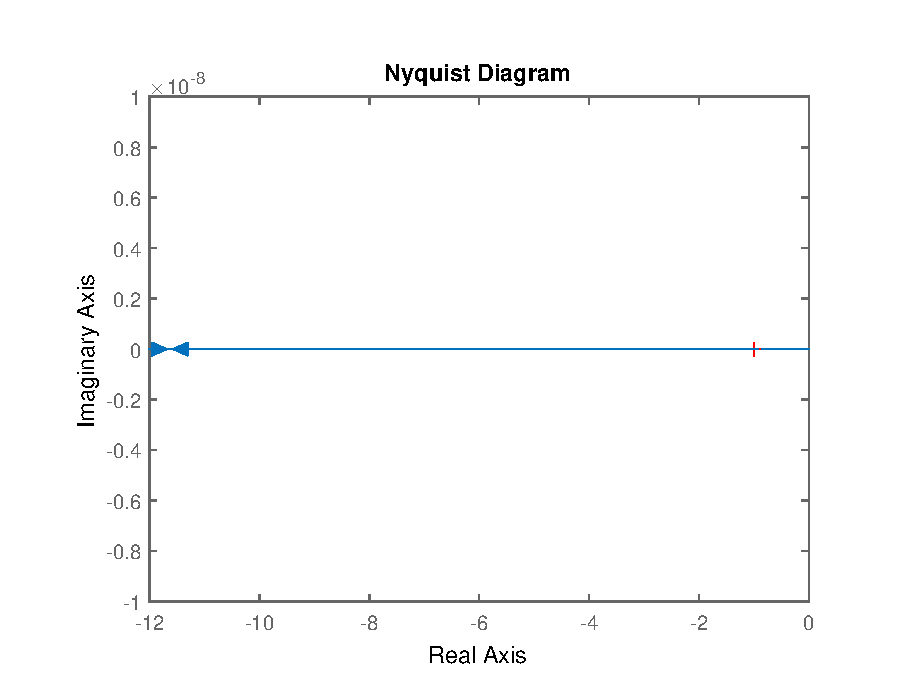
\includegraphics[scale=0.5]{fig1.eps}
		\caption{Nyquist plot for the double integrator system.}
	\end{figure}
	
	Examining the behaviour of the magnitude as $\omega \to 0$, we take the limit of equation (7):
	\begin{align*}
		\lim_{\omega\to 0}|G(j \omega)| = \lim_{\omega\to 0}\frac{1}{\omega^2} = \infty
	\end{align*}
	
	Examining the behaviour of the angle as $\omega \to 0$, we take the limit of equation (8):
	\begin{align*}
		\lim_{\omega\to 0}\angle G(j \omega) = 180 \si{\degree}
	\end{align*}
	
	Examining the behaviour of the magnitude as $\omega \to \infty$, we take the limit of equation (7):
	\begin{align*}
		\lim_{\omega\to 0}|G(j \omega)| = \lim_{\omega\to 0}\frac{1}{\omega^2} = 0
	\end{align*}
	
	Examining the behaviour of the angle as $\omega \to \infty$, we take the limit of equation (8):
	\begin{align*}
		\lim_{\omega\to 0}\angle G(j \omega) = 180 \si{\degree}
	\end{align*}
	
	The system itself is a double integrator, with the Nyquist plot passing directly through the critical -1 value: the system is inherently prone to \textit{blowing up}. It may be envisioned that a rocket which could employ an open loop control method which may help it to avoid this critical -1 value and provide safe flight, however, a rocket is a system that experiences many stochastic perturbations during flight. These perturbations could move the rocket output angle from the intended input reference. For this reason, an open loop control is not a suitable control method. Hence, the rocket requires feedback in order to control its path properly.\\
	
%%%%%%%%%%%%%%%%%%%%%%%%%%%%%%%%%%%%%%%%%%%%%%%%%%%%%%%%%%%%%%%%%%%%%%%%%%%%%%%%%%%%%%%%%%%%%%%%%%%%%%%%%%%%%%%%%%%%%%
% Question 2.4
%%%%%%%%%%%%%%%%%%%%%%%%%%%%%%%%%%%%%%%%%%%%%%%%%%%%%%%%%%%%%%%%%%%%%%%%%%%%%%%%%%%%%%%%%%%%%%%%%%%%%%%%%%%%%%%%%%%%%%


    \textbf{Question 2.4}\\
    
    A block doagram of the controlled system in the Laplace domain can be seen in Figure 1. We note that $G_P(s) = K(\tau s + 1)$, and $G_C(s) = \sfrac{1}{s^2}$.
    
    % Draw a simple picture of the pump tank system use this section to calculate the cross sectional area of the device.
    \tikzstyle{block} = [draw, fill=blue!20, rectangle, 
    minimum height=3em, minimum width=6em]
    \tikzstyle{sum} = [draw, fill=blue!20, circle, node distance=1cm]
    \tikzstyle{input} = [coordinate]
    \tikzstyle{output} = [coordinate]
    \tikzstyle{pinstyle} = [pin edge={to-,thin,black}]
    
    \begin{figure}[H]
    	\centering
    	% The block diagram code is probably more verbose than necessary
    	\begin{tikzpicture}[auto, node distance=2cm,>=latex']
    	% We start by placing the blocks
    	\node [input, name=input] {};
    	\node [sum, right of=input] (sum) {};
    	\node [block, right of=sum] (controller) {$G_C(s)$};
    	\node [block, right of=controller, node distance=3cm] (system) {$G_P(s)$};
    	% We draw an edge between the controller and system block to 
    	% calculate the coordinate u. We need it to place the measurement block. 
    	\draw [->] (controller) -- node[name=u] {$A(s)$} (system);
    	\node [output, right of=system] (output) {};
    	\node [below of=u] (measurements) {};
    	
    	% Once the nodes are placed, connecting them is easy. 
    	\draw [draw,->] (input) -- node {$R(s)$} (sum);
    	\draw [->] (sum) -- node {$E(s)$} (controller);
    	\draw [->] (system) -- node [name=y] {$\Phi(s)$}(output);
    	\draw [-] (y) |- (measurements.center);
    	\draw [->] (measurements.center) -| node[pos=0.99] {$-$} 
    	node [near end] {} (sum);
    	\end{tikzpicture}
    	\caption{Closed Loop Feedback Control for Rocket System}
    \end{figure}
    
    The transfer function, $G_{open loop}(s)$, for the open loop control system, when $\tau = 1$, can be seen below. This is simply the controller and the system without the feedback loop:
    \begin{align*}
	    G_{0}(s) 	&= G_P(s) \cdot G_C(s)\\
					&= \frac{K \cdot (s + 1)}{s^2}
    \end{align*}
    
    The Nyquist plot of the system, for $K=1$ and $K=2$, can be seen from the Matlab plot below:
    \begin{figure}[h]
    	\centering
    	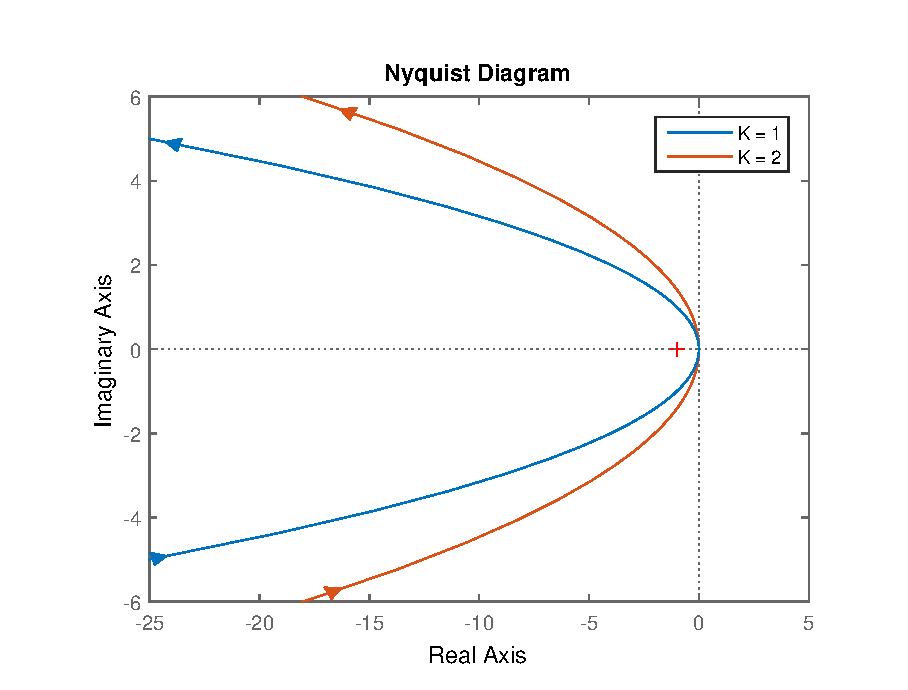
\includegraphics[scale=0.5]{fig2.eps}
    	\caption{Nyquist plot the the open loop controlled system}
    \end{figure}
	
	We can provide an analysis of the Nyquist plot by considering the magnitude and phase of the open loop transfer function as the frequency approaches zero and infinity. First, the magnitude of $G_0(j \omega)$ is:
	\begin{align}
		|G_0(j \omega)| = \bigg|\frac{jK \omega + K}{- \omega^2}\bigg| = \sqrt{\frac{K^2}{\omega^4} + \frac{K^2}{\omega^2}}
	\end{align}
	
	The phase of $G_0(j \omega)$ is given as follows:
	\begin{align}
		\angle G_0(j \omega) = \frac{\angle (jK \omega + K)}{\angle - \omega^2} = \angle (jK \omega + K) - \angle - \omega^2 = \angle (jK \omega + K) - 180 \si{\degree}
	\end{align}
	
	Examining the behaviour of the magnitude as $\omega \to 0$, we take the limit of equation (9):
	\begin{align*}
	\lim_{\omega\to 0}|G_0(j \omega)| = \lim_{\omega\to 0}\sqrt{\frac{K^2}{\omega^4} + \frac{K^2}{\omega^2}} = \infty
	\end{align*}
	
	Examining the behaviour of the angle as $\omega \to 0$, we take the limit of equation (10):
	\begin{align*}
	\lim_{\omega\to 0}\angle G_0(j \omega) = \lim_{\omega\to 0}\angle (jK \omega + K) - 180 \si{\degree} = -180 \si{\degree}
	\end{align*}
	
	Examining the behaviour of the magnitude as $\omega \to \infty$, we take the limit of equation (9):
	\begin{align*}
	\lim_{\omega\to \infty}|G_0(j \omega)| = \lim_{\omega\to 0}\sqrt{\frac{K^2}{\omega^4} + \frac{K^2}{\omega^2}} = 0
	\end{align*}
	
	Examining the behaviour of the angle as $\omega \to \infty$, we take the limit of equation (10):
	\begin{align*}
	\lim_{\omega\to \infty}\angle G_0(j \omega) = \lim_{\omega\to \infty}\angle (jK \omega + K) - 180 \si{\degree} = -90 \si{\degree}
	\end{align*}
	
	Suppose the controller was a P controller, the transfer function for the controller would be $G_C(s) = K$. The overall transfer function for the system and controller would be:
	\begin{align*}
		G(s) = G_P(s) \cdot G_C(s) = \frac{K}{s^2}
	\end{align*}
	
	This control method does not abate the inherent instability present in the system we are trying to control, that is the controller plus the system has a transfer function which behaves as a double integrator still. Hence, it will not be possible to control the system with a P controller. If the controller was an I controller, the transfer function would be $G_C(s) = \frac{K}{s}$. The overall transfer function for the system and controller would be:
	\begin{align*}
		G(s) = \frac{K}{s^3}
	\end{align*}
	
	Letting $s = j \omega$, we see that the transfer function becomes:
	\begin{align*}
		G(j \omega) = \frac{K}{-j \omega^3} = j \frac{K}{\omega^3}
	\end{align*}
	
	The magnitude of the transfer function is given by:
	\begin{align*}
		|G(j \omega)| = \frac{K}{\omega^3}
	\end{align*}
	
	The phase of the transfer function is given by:
	\begin{align*}
		\angle G(j \omega) = 90\si{\degree}
	\end{align*}
	
	Examining the behaviour of the magnitude as $\omega \to 0$, we take the limit of the magnitude function:
	\begin{align*}
	\lim_{\omega\to 0}|G(j \omega)| = \infty
	\end{align*}
	
	Examining the behaviour of the angle as $\omega \to 0$, we take the limit of the phase function:
	\begin{align*}
	\lim_{\omega\to 0}\angle G(j \omega) = 90 \si{\degree}
	\end{align*}
	
	Examining the behaviour of the magnitude as $\omega \to \infty$, we take the limit of the magnitude function:
	\begin{align*}
	\lim_{\omega\to \infty}|G(j \omega)| = 0
	\end{align*}
	
	Examining the behaviour of the angle as $\omega \to \infty$, we take the limit of the phase function:
	\begin{align*}
	\lim_{\omega\to \infty}\angle G(j \omega) = 90 \si{\degree}
	\end{align*}
	
	Hence, the Nyquist plot runs along the imaginary axis, and doesn't touch -1. Therefore the system cold be controlled using an open loop I controller, provided there were no stochastic perturbations interfering with the system.\\
%%%%%%%%%%%%%%%%%%%%%%%%%%%%%%%%%%%%%%%%%%%%%%%%%%%%%%%%%%%%%%%%%%%%%%%%%%%%%%%%%%%%%%%%%%%%%%%%%%%%%%%%%%%%%%%%%%%%%%
% Question 2.5
%%%%%%%%%%%%%%%%%%%%%%%%%%%%%%%%%%%%%%%%%%%%%%%%%%%%%%%%%%%%%%%%%%%%%%%%%%%%%%%%%%%%%%%%%%%%%%%%%%%%%%%%%%%%%%%%%%%%%%
	
	\textbf{Question 2.5}\\
	
    Making reference to Figure 1, we note that the output of the system can be expressed as:
    \begin{align}
	    \Phi(s) = G_C(s) \cdot G_P(s) \cdot E(s)
    \end{align}
	
	Further, by inspection, we can see that the error between the output and the input reference signal is given by:
	\begin{align}
		E(s) = R(s) - \Phi(s)
	\end{align}
	
	Substituting equation (12) into equation (11), we get that:
	\begin{align*}
		\Phi(s) = G_C(s) \cdot G_P(s) \cdot \bigg( R(s) - \Phi(s) \bigg)
	\end{align*}
	
	Rearranging, we see:
	\begin{align*}
		\Phi(s) \cdot \bigg( 1 + G_P(s) \cdot G_C(s) \bigg) = G_P(s) \cdot G_C(s) \cdot R(s)
	\end{align*}
	
	The transfer function for the closed loop system, $G_1(s)$, is given by:
	\begin{align}
		G_1(s) = \frac{\Phi(s)}{R(s)} = \frac{G_P(s) \cdot G_C(s}{1 + G_P(s) \cdot G_C(s)}
	\end{align}
	
	Using our expression for the controller, $G_C(s) = K \cdot (s + 1)$, and the expression for the system itself, $G_P(s) = \sfrac{1}{s^2}$, we see that the actual transfer function is defined as follows:
	\begin{align}
		G_1(s) 	&= \frac{\frac{1}{s^2} \cdot K \cdot (s + 1)}{1 + \frac{1}{s^2} \cdot K \cdot (s + 1)} \nonumber \\
				&= \frac{Ks + K}{s^2 + Ks + K}
	\end{align}
	
	If $K = 1$, then the closed loop transfer function becomes:
	\begin{align*}
		G_1(s) = \frac{s + 1}{s^2 + s + 1}
	\end{align*}
	
	The zeros of the transfer function in this instance, are given found when $s + 1 = 0$, that is when $s = -1$. The poles of the transfer function are found when $s^2 + s + 1 = 0$, that is when $s = -0.5 \pm j0.87$.
	
	If $K = 2$, then the closed loop transfer function becomes:
	\begin{align*}
		G_1(s) = \frac{2s + 2}{s^2 + 2s + 21}
	\end{align*}
	
	The zeros of the transfer function in this instance, are given found when $2s + 2 = 0$, that is when $s = -1$. The poles of the transfer function are found when $s^2 + 2s + 2 = 0$, that is when $s = -1 \pm j$.\\
	
	It may be hypothesised that the zeros are independent of the value of $K$. A short proof using the general transfer function seen in equation (14) starts with setting the numerator to zero> This gives us $Ks + K = 0$. Solving for $s$, we see that $s = -\frac{K}{K}$ = -1. Hence, the zeros of the transfer function $G_1(s)$ are independent of the value of $K$. To determine the steady state response of the closed loop system in the time domain, when the input is a unit step function we employ the use of the final value theorem:
	\begin{align*}
		\lim_{t \to \infty} \phi(t) 	& = \lim_{s \to 0} s \cdot \Phi(s)\\
										& = \lim_{s \to 0} s \cdot G_1(s) \cdot R(s)\\
										&= \lim_{s \to 0} s \cdot \bigg[ \frac{K(s + 1)}{s^2 + Ks +K}\bigg] \cdot R(s)
	\end{align*}
	
	We note that the Laplace transform of the unit step function is $\frac{1}{s}$. Hence, we get that:
	\begin{align*}
		\lim_{t \to \infty} \phi(t) &= \lim_{s \to 0} s \cdot \bigg[ \frac{K(s + 1)}{s^2 + Ks +K}\bigg] \cdot \frac{1}{s}\\
									&= \lim_{s \to 0} \frac{K(s + 1)}{s^2 + Ks +K}\\
									&= \frac{K}{K}\\
									&= 1
	\end{align*}
	
	This means that as the system tends to an infinite time horizon, the error between the input reference and the output signal tends to zero. The output of the system converges to the input.\\
	\newpage
	
%%%%%%%%%%%%%%%%%%%%%%%%%%%%%%%%%%%%%%%%%%%%%%%%%%%%%%%%%%%%%%%%%%%%%%%%%%%%%%%%%%%%%%%%%%%%%%%%%%%%%%%%%%%%%%%%%%%%%%
% Question 2.6
%%%%%%%%%%%%%%%%%%%%%%%%%%%%%%%%%%%%%%%%%%%%%%%%%%%%%%%%%%%%%%%%%%%%%%%%%%%%%%%%%%%%%%%%%%%%%%%%%%%%%%%%%%%%%%%%%%%%%%

	\textbf{Question 2.6}\\
	
	A Matlab script, which can be seen in Appendix A, was created to simulate a step response to the controlled system with $K = 1$, and $\tau = 1$. The script was run subsequently, using different values of $K$, to find the first point at which the system overshoot reached 25\%. The parameter which achieved the 25\% overshoot was $K = 1.427$. A plot of the the system output, $\phi(t)$, can be seen in Figure 3, in addition to the errors in the system, $e(t)$, and the reference signal, $r(t)$.
	
	\begin{figure}[h]
		\centering
		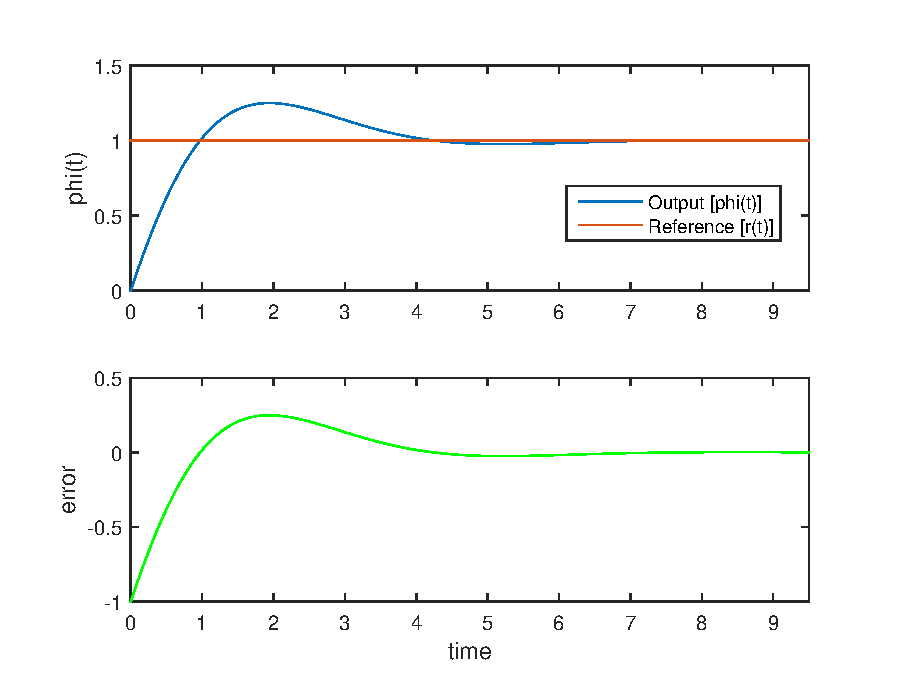
\includegraphics[scale=0.8]{fig3.eps}
		\caption{The figure shows step input response in the time domain, and error signal converging to zero.}
	\end{figure}
	
	The rise time of the system is approximately 1 second, which was found by inspection from the graph.\\
	
	\newpage
%%%%%%%%%%%%%%%%%%%%%%%%%%%%%%%%%%%%%%%%%%%%%%%%%%%%%%%%%%%%%%%%%%%%%%%%%%%%%%%%%%%%%%%%%%%%%%%%%%%%%%%%%%%%%%%%%%%%%%
% Question 2.7
%%%%%%%%%%%%%%%%%%%%%%%%%%%%%%%%%%%%%%%%%%%%%%%%%%%%%%%%%%%%%%%%%%%%%%%%%%%%%%%%%%%%%%%%%%%%%%%%%%%%%%%%%%%%%%%%%%%%%%

	\textbf{Question 2.7}\\
	
	The Matlab script previously referenced in Appendix A also creates a Bode plot of the transfer function which maps the reference signal, $R(j \omega)$, to the system output, $\Phi(j \omega)$. The Bode plot can be seen in Figure 3. The maximum overshoot in the frequency domain is approximately 34\%, by inspection from the graph.
	
	\begin{figure}[h]
		\centering
		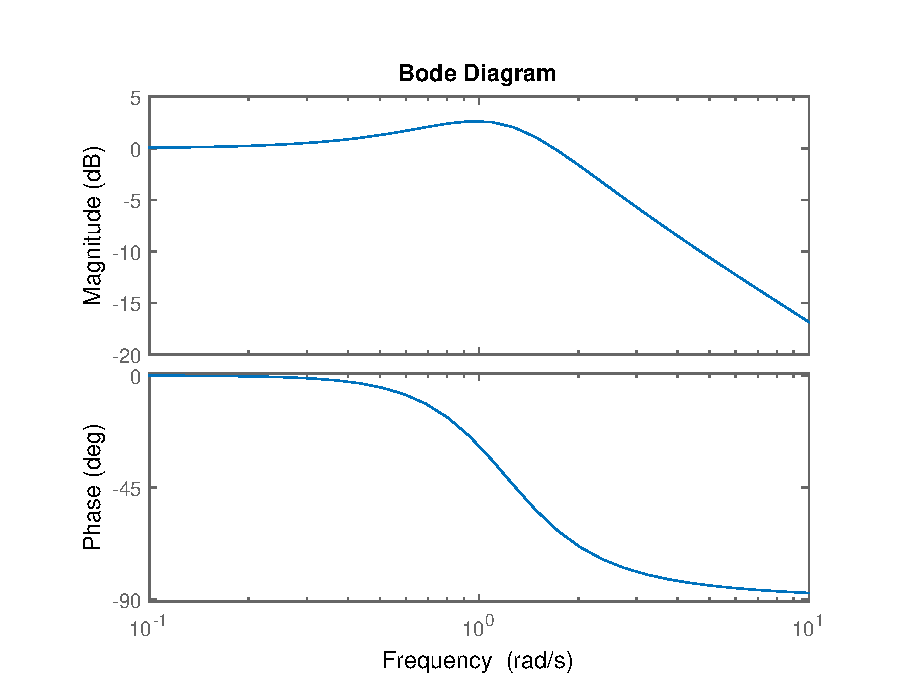
\includegraphics[scale=0.8]{fig4.eps}
	\end{figure}
	
	\newpage
%%%%%%%%%%%%%%%%%%%%%%%%%%%%%%%%%%%%%%%%%%%%%%%%%%%%%%%%%%%%%%%%%%%%%%%%%%%%%%%%%%%%%%%%%%%%%%%%%%%%%%%%%%%%%%%%%%%%%%
% Appendix A
%%%%%%%%%%%%%%%%%%%%%%%%%%%%%%%%%%%%%%%%%%%%%%%%%%%%%%%%%%%%%%%%%%%%%%%%%%%%%%%%%%%%%%%%%%%%%%%%%%%%%%%%%%%%%%%%%%%%%%
	
	\textbf{Appendix A}\\
	
	The Matlab code which was used in questions 2.6 and 2.7 is shown below:
	
	\begin{lstlisting}
		% Clear variables and the workspace
		clear; clc;
		
		% Set model parameters
		T = 1;
		K = 1.427;
		
		% Define the numberator and denominator for the transfer function
		numerator = [K*T K];
		denominator = [1 K K];
		
		% Build transfer function
		sys = tf(numerator,denominator);
		
		% Step response to closed loop controlled system
		[phi,time] = step(sys);
		step_plot = ones(length(phi),1);
		error_plot = phi - step_plot;
		Mo = ((max(phi) - 1)/1)*100;
		
		% Print the maxover shoot in time domain
		fprintf('Max overshoot: %.2f\n',Mo);
		
		% Plot step response
		figure(1)
		subplot(2,1,1)
		plot(time, phi,time,step_plot)
		ylabel('phi(t)')
		axis([0,9.5,0,1.5])
		legend('Output [phi(t)]','Reference [r(t)]')
		
		subplot(2,1,2)
		plot(time, error_plot,'g')
		xlabel('time')
		ylabel('error')
		axis([0,9.5,-1,0.5])
		
		% Plot bode plot
		figure(2)
		bode(sys)
	\end{lstlisting}
	
\end{document}
